% Propósito: distinguir las transformaciones físicas de audífono, implante
% coclear y dispositivo de conducción ósea.
% Origen: secciones \ref{sec:u8-audifonos}, \ref{sec:u8-implantes} y
% \ref{sec:u8-conduccion-osea}, más la notación de presión p(t), corriente i(t)
% y desplazamiento xi(t). Esquema funcional; no representa marcas, anatomía,
% estrategias de codificación, ganancias ni indicaciones clínicas.
% Descripción accesible: tres filas parten de presión acústica en pascales y
% pasan por micrófono y procesamiento eléctrico. El audífono usa un receptor y
% vuelve a producir presión acústica cerca del oído. El implante usa un enlace,
% estimulador y electrodos para producir corriente eléctrica en la cóclea. El
% dispositivo de conducción ósea usa un vibrador para producir desplazamiento
% mecánico en el cráneo. Los sombreados separan dominios acústico, eléctrico y
% mecánico.
% Validación prevista: comprobar que las tres entradas son acústicas, que las
% salidas se expresan como p(t) en Pa, i(t) en A y xi(t) en m, que el implante
% no aparece como amplificador acústico, que la vía ósea no se dibuja hacia
% una única cóclea y que las flechas conserven una separación visible entre
% bloques al ancho final de página.
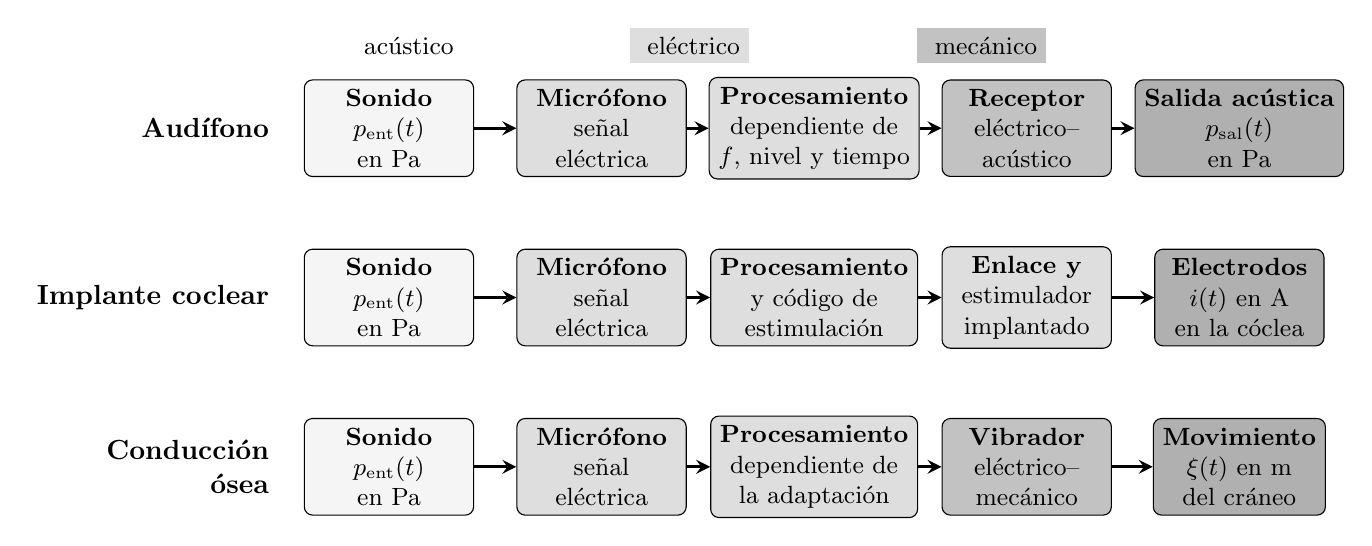
\begin{tikzpicture}[font=\small,>=stealth,x=1cm,y=1cm]
    \tikzset{
        block/.style={
            draw,rounded corners=3pt,
            minimum width=2.15cm,minimum height=1.05cm,
            align=center
        },
        acoustic/.style={block,fill=black!4},
        electric/.style={block,fill=black!13},
        mechanical/.style={block,fill=black!24},
        output/.style={block,fill=black!31},
        flow/.style={->,very thick}
    }

    \node[font=\bfseries,anchor=east] at (0.15,5.10) {Audífono};
    \node[acoustic] (ha-in) at (1.55,5.10)
        {\textbf{Sonido}\\\(p_\mathrm{ent}(t)\)\\en Pa};
    \node[electric] (ha-mic) at (4.25,5.10)
        {\textbf{Micrófono}\\señal\\eléctrica};
    \node[electric] (ha-proc) at (6.95,5.10)
        {\textbf{Procesamiento}\\dependiente de\\\(f\), nivel y tiempo};
    \node[mechanical] (ha-rec) at (9.65,5.10)
        {\textbf{Receptor}\\eléctrico--\\acústico};
    \node[output] (ha-out) at (12.35,5.10)
        {\textbf{Salida acústica}\\\(p_\mathrm{sal}(t)\)\\en Pa};

    \node[font=\bfseries,anchor=east] at (0.15,2.95) {Implante coclear};
    \node[acoustic] (ci-in) at (1.55,2.95)
        {\textbf{Sonido}\\\(p_\mathrm{ent}(t)\)\\en Pa};
    \node[electric] (ci-mic) at (4.25,2.95)
        {\textbf{Micrófono}\\señal\\eléctrica};
    \node[electric] (ci-proc) at (6.95,2.95)
        {\textbf{Procesamiento}\\y código de\\estimulación};
    \node[electric] (ci-link) at (9.65,2.95)
        {\textbf{Enlace y}\\estimulador\\implantado};
    \node[output] (ci-out) at (12.35,2.95)
        {\textbf{Electrodos}\\\(i(t)\) en A\\en la cóclea};

    \node[font=\bfseries,anchor=east,align=right] at (0.15,0.80)
        {Conducción\\ósea};
    \node[acoustic] (bc-in) at (1.55,0.80)
        {\textbf{Sonido}\\\(p_\mathrm{ent}(t)\)\\en Pa};
    \node[electric] (bc-mic) at (4.25,0.80)
        {\textbf{Micrófono}\\señal\\eléctrica};
    \node[electric] (bc-proc) at (6.95,0.80)
        {\textbf{Procesamiento}\\dependiente de\\la adaptación};
    \node[mechanical] (bc-vib) at (9.65,0.80)
        {\textbf{Vibrador}\\eléctrico--\\mecánico};
    \node[output] (bc-out) at (12.35,0.80)
        {\textbf{Movimiento}\\\(\xi(t)\) en m\\del cráneo};

    \foreach \a/\b in {
        ha-in/ha-mic,ha-mic/ha-proc,ha-proc/ha-rec,ha-rec/ha-out,
        ci-in/ci-mic,ci-mic/ci-proc,ci-proc/ci-link,ci-link/ci-out,
        bc-in/bc-mic,bc-mic/bc-proc,bc-proc/bc-vib,bc-vib/bc-out}{
        \draw[flow] (\a.east) -- (\b.west);
    }

    \node[anchor=west] at (1.00,6.15)
        {\(\square\) acústico};
    \node[anchor=west,fill=black!13] at (4.60,6.15)
        {\(\square\) eléctrico};
    \node[anchor=west,fill=black!24] at (8.25,6.15)
        {\(\square\) mecánico};
\end{tikzpicture}
